\section*{Exercice 144 -- Train épicycloïdal}

\setcounter{exo}{0}

\ifprof
\else
Soit le train épicycloïdal suivant. 

\begin{center}
 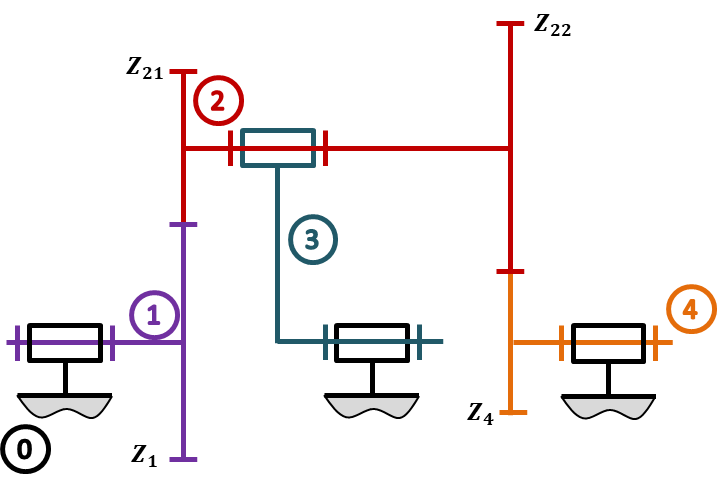
\includegraphics[width=.6\linewidth]{TrainEpi_04.png}
\end{center}
\fi

\ifprof
\newpage
\else
\fi

\subparagraph{}
\textit{Déterminer $\omega_{40}$ en fonction de  $\omega_{30}$ et $\omega_{10}$.}
\ifprof
 \begin{corrige}
 
 En bloquant le porte satellite, on a : $\dfrac{\omega_{43}}{\omega_{13}}=\dfrac{Z_{1}Z_{22}}{Z_{21}Z_{4}}$.
  On a donc, 
  $\dfrac{\omega_{40}+\omega_{03}}{\omega_{10}+\omega_{03}}=
\dfrac{Z_{1}Z_{22}}{Z_{21}Z_{4}}$

  $\Leftrightarrow \omega_{40}+\omega_{03}=\dfrac{Z_{1}Z_{22}}{Z_{21}Z_{4}}\left( \omega_{10}+\omega_{03} \right)$
 
 $\Leftrightarrow \omega_{40}=\dfrac{Z_{1}Z_{22}}{Z_{21}Z_{4}}\left( \omega_{10}-\omega_{30} \right) + \omega_{30}$

 $\Leftrightarrow \omega_{40}=\dfrac{Z_{1}Z_{22}}{Z_{21}Z_{4}}\omega_{10} +\left(1- \dfrac{Z_{1}Z_{22}}{Z_{21}Z_{4}}\right)\omega_{30}$

 \end{corrige}
 \else
 \fi
 
\subparagraph{}
\textit{On suppose que $\omega_{40}$ est bloqué. Exprimer le rapport $\dfrac{\omega_{30}}{\omega_{10}}$.}
\ifprof
 \begin{corrige}
 $\Leftrightarrow 0=\dfrac{Z_{1}Z_{22}}{Z_{21}Z_{4}}\omega_{10} +\left(1- \dfrac{Z_{1}Z_{22}}{Z_{21}Z_{4}}\right)\omega_{30}$

$\Leftrightarrow  \dfrac{Z_{1}Z_{22}}{Z_{21}Z_{4}}\omega_{10} =-\left(1- \dfrac{Z_{1}Z_{22}}{Z_{21}Z_{4}}\right)\omega_{30}$

$\Leftrightarrow  \dfrac{\omega_{30}}{\omega_{10}} = \dfrac{ \dfrac{Z_{1}Z_{22}}{Z_{21}Z_{4}}}{ \dfrac{Z_{1}Z_{22}}{Z_{21}Z_{4}}-1}= \dfrac{ {Z_{1}Z_{22}}}{ {Z_{1}Z_{22}}-Z_{21}Z_{4}}$
 \end{corrige}
 \else
 \fi

